% 03_methods.tex
% 方法部分

本节详细介绍谱-时序 Transformer 的架构设计、面向扩展性的设计考量以及训练策略。

\subsection{问题形式化}
\label{subsec:problem_formulation}

给定图 $G$ 的拉普拉斯谱 $(\Lambda, U)$,目标是预测 FALQON 参数序列 $\bm{\beta} = (\beta_0, \beta_1, \ldots, \beta_{P-1})$。我们将此建模为条件序列生成问题:
\begin{equation}
p(\bm{\beta} | G) = \prod_{t=0}^{P-1} p(\beta_t | \beta_{<t}, G)
\end{equation}

\subsection{模型架构}
\label{subsec:architecture}

谱-时序 Transformer 包含三个核心模块:谱编码器、图全局表示和时序解码器。

\subsubsection{符号不变谱编码器(SignNet)}
\label{subsec:signnet}

为解决特征向量的符号模糊性,我们采用 SignNet 进行预处理。对于特征向量 $u_i$,SignNet 通过对称化操作消除符号歧义:
\begin{equation}
h_i = \rho\left( \phi(u_i) + \phi(-u_i) \right)
\end{equation}
其中 $\phi: \mathbb{R}^n \to \mathbb{R}^d$ 为多层感知机(MLP),$\rho: \mathbb{R}^d \to \mathbb{R}^d$ 为聚合层。该设计保证 $h_i = h_{-u_i}$,从而消除符号歧义。

特征值通过独立的 MLP 编码:
\begin{equation}
e_i = \text{MLP}_{\lambda}(\lambda_i)
\end{equation}

两者通过融合层结合,得到谱模态表示:
\begin{equation}
m_i = \text{Fusion}\left( e_i, h_i \right) = \text{Linear}([e_i; h_i])
\end{equation}

\subsubsection{图全局表示}

为了捕捉图的整体特性,我们引入可学习的图全局 token。通过对有效谱模态的聚合,计算图的全局嵌入:
\begin{equation}
g = \frac{1}{N} \sum_{i=1}^{N} m_i
\end{equation}
该全局嵌入与可学习的 token 嵌入结合后,作为 Transformer 解码器的第一个 memory 位置。

\subsubsection{时序解码器}

采用标准 Transformer Decoder \cite{vaswani2017attention},Query 由三部分组成:
\begin{equation}
q_t = e_{\text{query}} + \text{PE}(t) + \text{Embed}(\beta_{t-1})
\end{equation}
其中:
\begin{itemize}
    \item $e_{\text{query}}$:可学习的查询嵌入
    \item $\text{PE}(t)$:正弦位置编码
    \item $\text{Embed}(\beta_{t-1})$:前一步预测值的嵌入(自回归)
\end{itemize}

解码器通过交叉注意力查询谱模态信息:
\begin{equation}
\text{CrossAttn}(Q, K, V) = \text{softmax}\left( \frac{QK^T}{\sqrt{d}} \right) V
\end{equation}
其中 $K, V$ 来自谱编码器输出(包括图全局 token 和谱模态),$Q$ 来自时序查询。

\subsubsection{输出头}

解码器输出经 MLP 映射为标量预测:
\begin{equation}
\hat{\beta}_t = \text{MLP}(\text{Decoder}(q_t, M))
\end{equation}

\subsection{面向扩展性的设计考量}
\label{subsec:scalability_design}

为使模型能够处理不同大小的图并实现跨规模泛化,我们在架构设计中融入以下考量:

\paragraph{谱特征的尺寸不变性}
归一化拉普拉斯矩阵的特征值总是位于 $[0, 2]$ 区间,无论图的大小如何。这为神经网络提供了稳定的数值范围,无需针对不同 $N$ 进行缩放。

\paragraph{基于分布的注意力机制}
Transformer 的 Softmax 注意力是对所有谱模态归一化的:
\begin{equation}
\alpha_i = \frac{\exp(q \cdot k_i)}{\sum_{j=1}^{N} \exp(q \cdot k_j)}
\end{equation}
模型学习的是"关注哪一部分频谱"的分布权重,而非具体的特征值索引。当 $N$ 增大时,谱变得更密集,但其分布形态保持相似,因此注意力模式依然有效。

\paragraph{可变长度处理}
通过 padding 和 mask 机制,模型可以在同一批次中处理不同大小的图。对于超出训练时最大节点数的图,可以截断至固定维度或使用滑动窗口策略。

\subsection{训练策略}
\label{subsec:training}

\subsubsection{Scheduled Sampling}

自回归模型在训练时使用真实的前一步值 $\beta_{t-1}$,但推理时必须使用预测值 $\hat{\beta}_{t-1}$。这种训练-推理不一致会导致误差累积。

我们采用 Scheduled Sampling \cite{bengio2015scheduled} 缓解此问题:
\begin{equation}
\tilde{\beta}_{t-1} = \begin{cases}
\beta_{t-1}^{\text{true}} & \text{w.p. } 1 - \epsilon \\
\hat{\beta}_{t-1} & \text{w.p. } \epsilon
\end{cases}
\end{equation}
其中采样概率 $\epsilon$ 从 0 线性增长至 0.3。

\subsubsection{损失函数}

总损失由三部分组成:
\begin{equation}
\mathcal{L} = \mathcal{L}_{\text{MSE}} + \lambda_1 \mathcal{L}_{\text{temporal}} + \lambda_2 \mathcal{L}_{\text{tail}}
\end{equation}

\textbf{加权 MSE 损失}:后段时间步赋予更高权重
\begin{equation}
\mathcal{L}_{\text{MSE}} = \frac{1}{P} \sum_{t=0}^{P-1} w_t (\hat{\beta}_t - \beta_t)^2, \quad w_t = 1 + \frac{t}{P} \cdot (w_{\text{tail}} - 1)
\end{equation}

\textbf{时序梯度损失}:鼓励学习变化趋势
\begin{equation}
\mathcal{L}_{\text{temporal}} = \frac{1}{P-1} \sum_{t=1}^{P-1} \left( \Delta\hat{\beta}_t - \Delta\beta_t \right)^2
\end{equation}
其中 $\Delta\beta_t = \beta_t - \beta_{t-1}$。

\subsection{复杂度分析}
\label{subsec:complexity}

表 \ref{tab:complexity} 对比了不同方法的量子和经典复杂度。

\begin{table}[htbp]
\centering
\caption{复杂度对比分析}
\label{tab:complexity}
\begin{tabular}{lccc}
\toprule
方法 & 量子电路执行次数 & 经典计算 & 对 $N$ 的依赖 \\
\midrule
原始 FALQON & $O(P^2)$ & $O(1)$ & 若 $P \propto N$,则 $O(N^2)$ \\
标准 QAOA & $O(k \cdot P)$ & $O(k)$ & $k$ 随 $N$ 指数增长 \\
\textbf{Neural-FALQON(本文)} & $O(1)$ & $O(N^3)$ & 经典 $O(N^3)$,量子 $O(1)$ \\
\bottomrule
\end{tabular}
\end{table}

\textbf{关键洞察}:我们用多项式级的经典算力($O(N^3)$ 的谱分解)换取了指数级昂贵的量子资源。对于 NISQ 时代的目标问题($N \sim 50-1000$),$N^3$ 的经典计算量在现代硬件上仅需秒级;相比之下,量子测量涉及硬件延迟、排队和高昂的单次运行费用。这体现了"混合量子-经典计算"的精髓。

\subsection{模型架构}
\label{subsec:architecture}

如图 \ref{fig:architecture} 所示,谱-时序 Transformer 包含三个核心模块。

\begin{figure}[htbp]
  \centering
  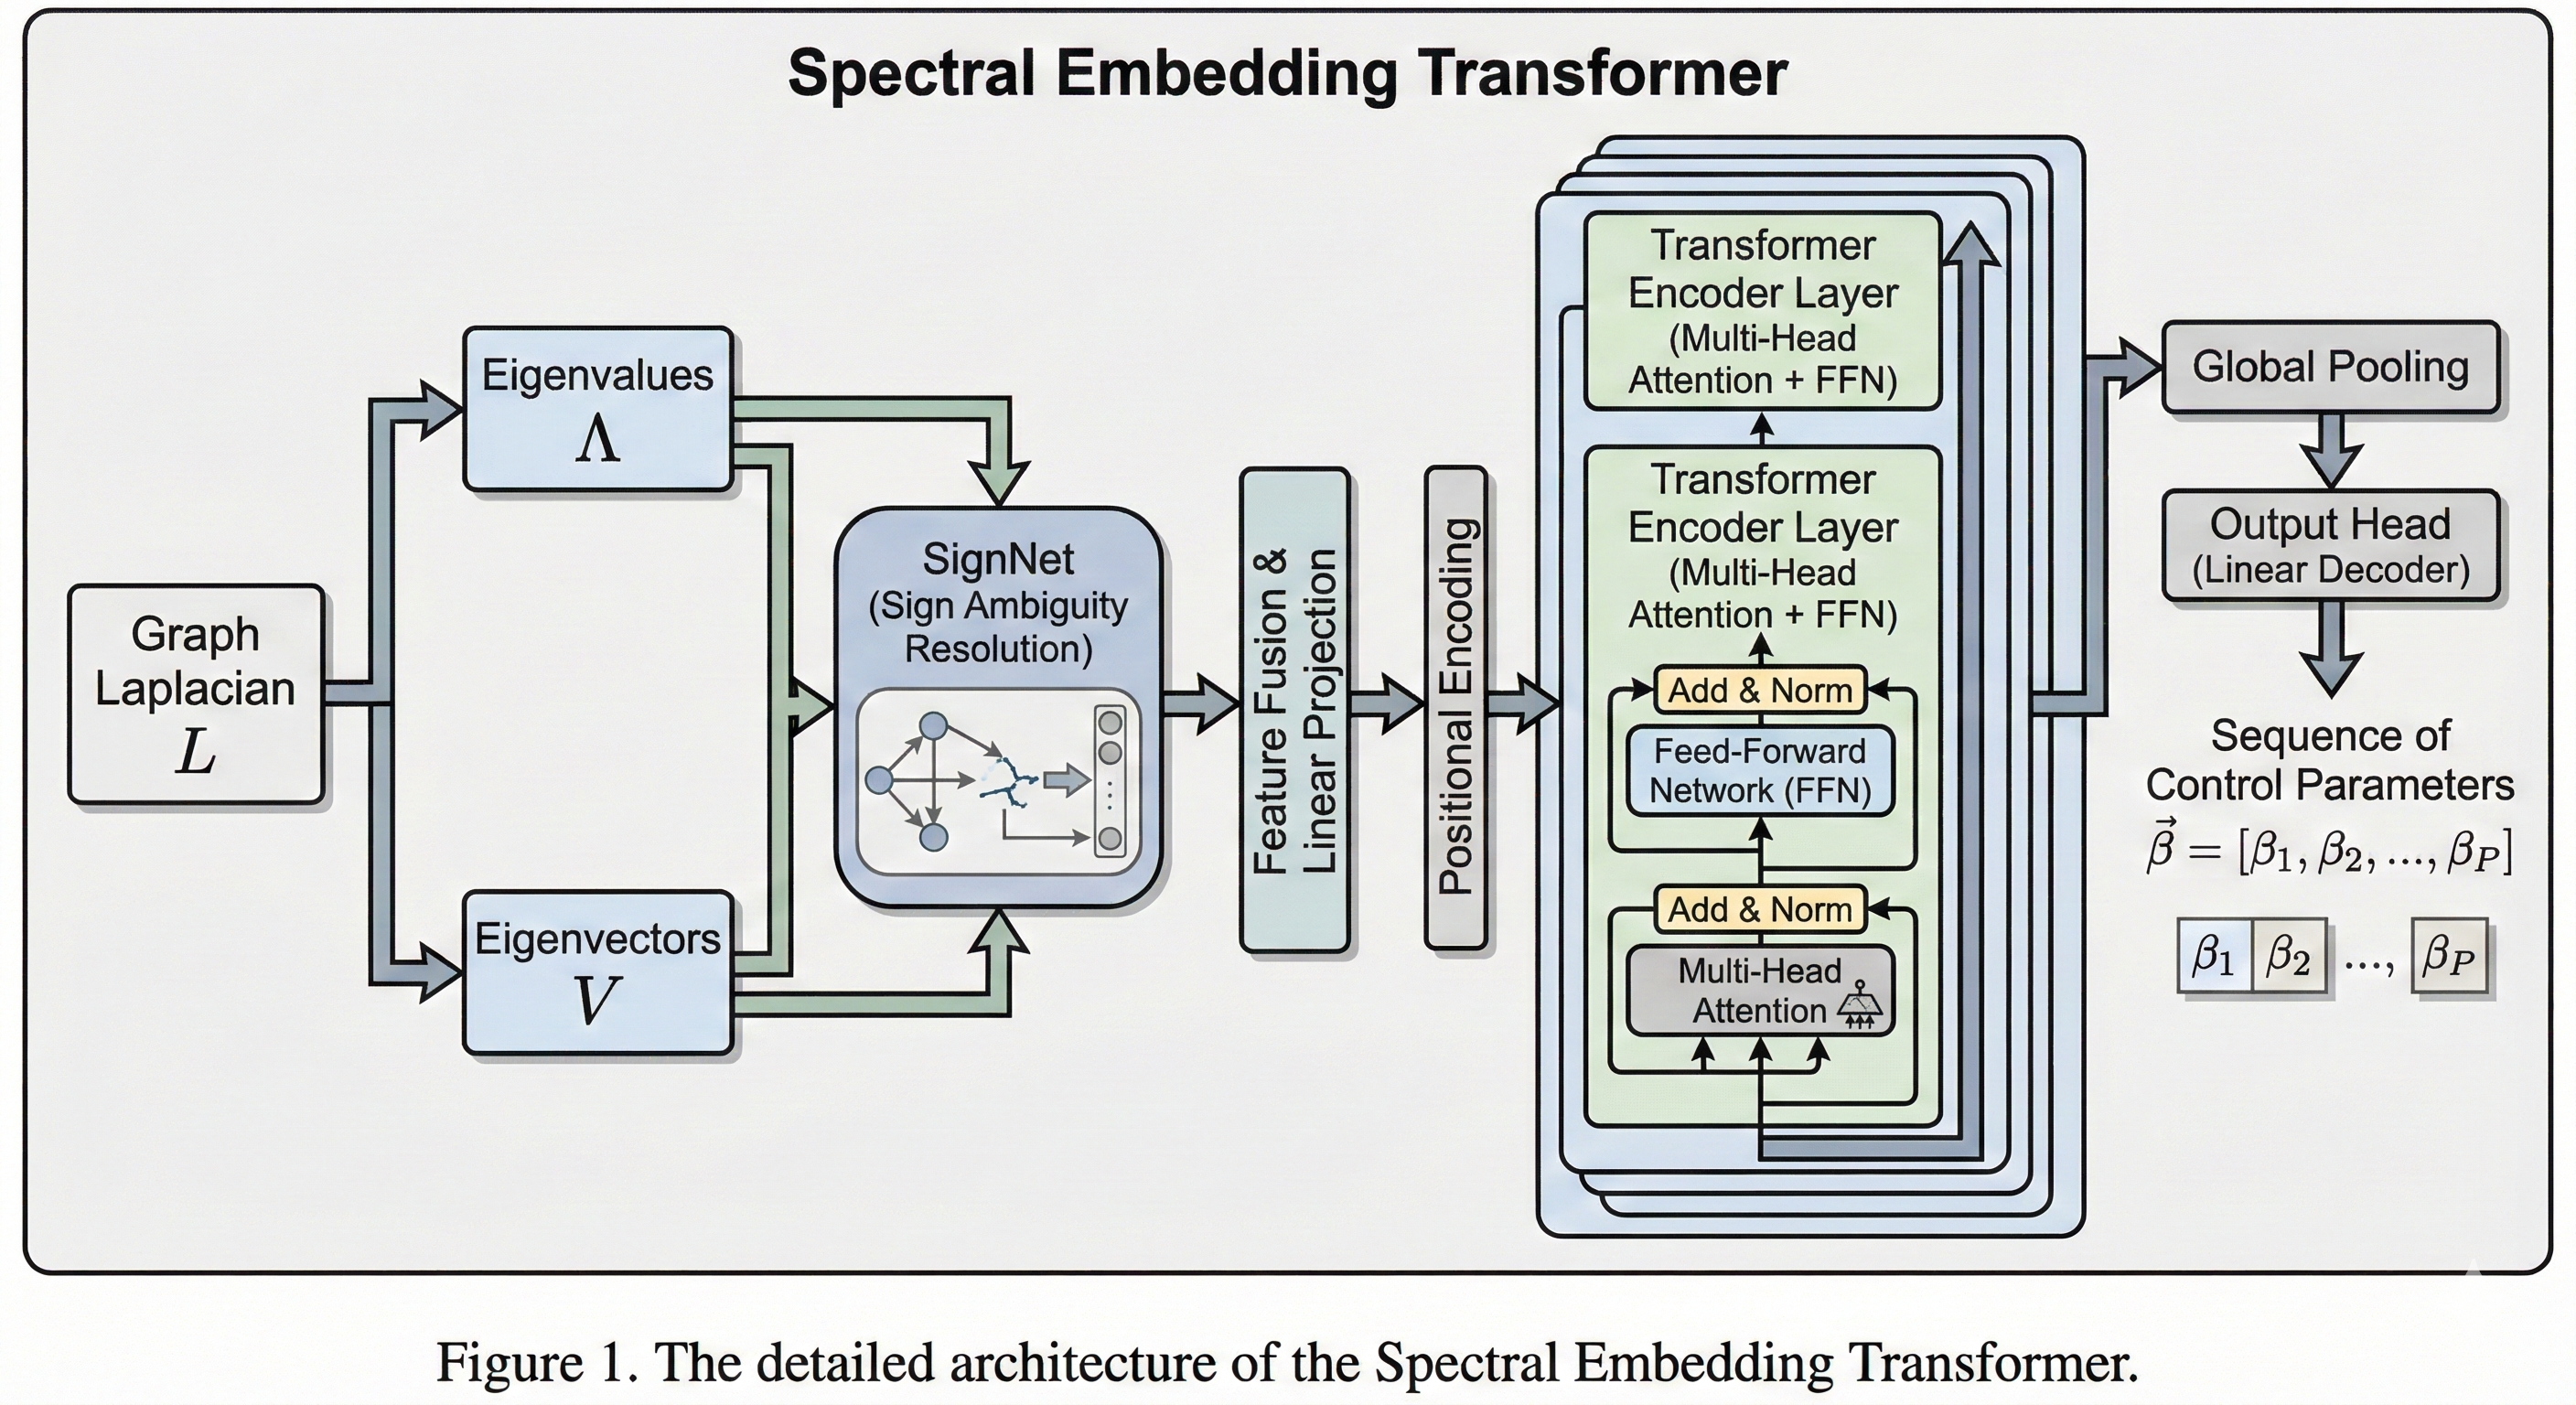
\includegraphics[width=0.9\linewidth]{figures/transformer_architecture.png}
  \caption{谱-时序 Transformer 的总体架构示意}
  \label{fig:architecture}
\end{figure}

\subsubsection{符号不变谱编码器(SignNet)}
\label{subsec:signnet}

为解决特征向量的符号模糊性,我们采用 SignNet 进行预处理:
\begin{equation}
h_i = \rho\left( \phi(u_i) + \phi(-u_i) \right)
\end{equation}
其中 $\phi: \mathbb{R}^n \to \mathbb{R}^d$ 为 MLP,$\rho: \mathbb{R}^d \to \mathbb{R}^d$ 为聚合层。该设计保证 $h_i = h_{-i}$,消除符号歧义。

特征值通过独立的 MLP 编码后与 SignNet 输出融合:
\begin{equation}
m_i = \text{Fusion}\left( \text{MLP}(\lambda_i), h_i \right)
\end{equation}
得到 $M$ 个谱模态的表示 $\{m_i\}_{i=1}^M$,作为 Transformer 解码器的 Memory。

\subsubsection{时序解码器}

采用标准 Transformer Decoder \cite{vaswani2017attention},Query 由时间步的正弦位置编码和前一步预测值的嵌入组成:
\begin{equation}
q_t = \text{PE}(t) + \text{Embed}(\beta_{t-1}) + e_{\text{query}}
\end{equation}
其中 $e_{\text{query}}$ 为可学习的查询嵌入。

解码器通过交叉注意力查询谱模态信息:
\begin{equation}
\text{CrossAttn}(Q, K, V) = \text{softmax}\left( \frac{QK^T}{\sqrt{d}} \right) V
\end{equation}
其中 $K, V$ 来自谱编码器输出,$Q$ 来自时序查询。

\subsubsection{输出头}

解码器输出经 MLP 映射为标量预测:
\begin{equation}
\hat{\beta}_t = \text{MLP}(\text{Decoder}(q_t, M))
\end{equation}

\subsection{训练策略}
\label{subsec:training}

\subsubsection{Scheduled Sampling}

为缓解训练(使用真实 $\beta_{t-1}$)与推理(使用预测 $\hat{\beta}_{t-1}$)的不一致,我们采用 Scheduled Sampling \cite{bengio2015scheduled}:
\begin{equation}
\tilde{\beta}_{t-1} = \begin{cases}
\beta_{t-1}^{\text{true}} & \text{w.p. } 1 - \epsilon \\
\hat{\beta}_{t-1} & \text{w.p. } \epsilon
\end{cases}
\end{equation}
其中 $\epsilon$ 从 0 线性增长至 0.3。

\subsubsection{损失函数}

总损失由三部分组成:
\begin{equation}
\mathcal{L} = \mathcal{L}_{\text{MSE}} + \lambda_1 \mathcal{L}_{\text{temporal}} + \lambda_2 \mathcal{L}_{\text{tail}}
\end{equation}

\begin{itemize}
    \item \textbf{加权 MSE}:后段时间步赋予更高权重
    \begin{equation}
    \mathcal{L}_{\text{MSE}} = \frac{1}{P} \sum_{t=0}^{P-1} w_t (\hat{\beta}_t - \beta_t)^2, \quad w_t = 1 + \frac{t}{P}
    \end{equation}
    
    \item \textbf{时序梯度损失}:鼓励学习变化趋势
    \begin{equation}
    \mathcal{L}_{\text{temporal}} = \frac{1}{P-1} \sum_{t=1}^{P-1} \left( \Delta\hat{\beta}_t - \Delta\beta_t \right)^2
    \end{equation}
    
    \item \textbf{尾部方差损失}:约束后段的动态范围
\end{itemize}